\chapter{Standar Pengajuan}

Pada pengajuan kali ini. Setiap mahasiswa tingkat akhir wajib untuk menemui pembimbing untuk menyepakati judul, metode, sumber data, abstrack dan referensi yang akan digunakan dalam penelitian. Sebelum pertemuan dengan pembimbing, mahasiswa wajib sudah membuat resume dari 15 jurnal dalam 5 tahun terakhir yang terindex scopus(cek di scimagojr.com) dan dituangkan di template presentasi. Template presentasi terdapat di situs informatika. Mahasiswa wajib melakukan presentasi terlebih dahulu ke pembimbing dengan template presentasi kemudian baru melakukan diskusi.Pengajuan penelitian tingkat akhir(Intership II dan Tugas Akhir) dilakukan melalui formulir online yang diberikan dan diisi bersama dengan Pembimbing apabila sudah disepakati dan disetujui bersama pembimbing. Pengisian form menggunakan email poltekpos dari pembimbing. Pastikan sudah melakukan login dengan email poltekpos terlebih dahulu oleh pembimbing. Formulir bisa diakses pada laman situs if.poltekpos.ac.id. Perlu diperhatikan Formulir yang perlu diisi terdiri dari :
\begin{enumerate}
\item Judul yang diajukan dalam bahasa inggris
\item abstrack berbahasa inggris terdiri dari 150-250 kata.
\item ringkasan yang terdiri dari metode yang digunakan, Data Penilitian (sumber data yang digunakan dan jumlah data yang digunakan)
\item daftar referensi
\end{enumerate}
Dari point diatas perlu diperhatikan adalah standar pengisian form masing-masing. Pembimbing adalah pembimbing Internship 2 dan Tugas Akhir adalah pembimbing dari Internship I. Setiap mahasiswa tingkat akhir harus memperhatikan data dosen yang terdapat pada situs Informatika pada menu tim seperti terlihat pada gambar \ref{figure:timif}.
\begin{figure}[ht]
	\centerline{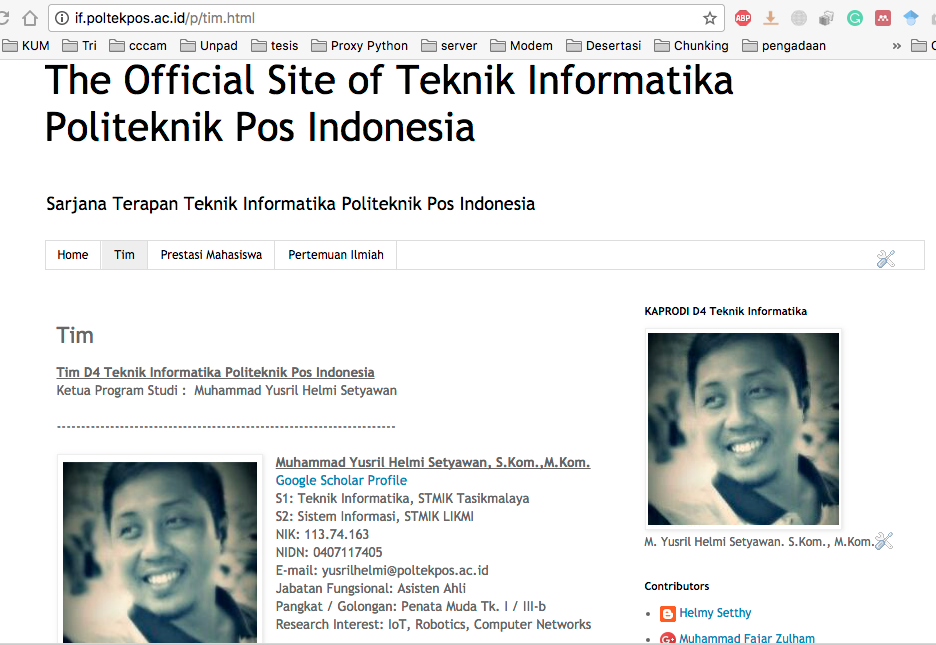
\includegraphics[width=0.5\textwidth]{figures/timif.png}}
	\caption{Data Pembimbing dari situs informatika.}
	\label{figure:timif}
	\end{figure}
Setiap mahasiswa wajib mematuhi aturan dari masing-masing pembimbing tentang tata cara komunikasi dan aturan bimbingan yang bisa diakses dari laman portal dosen masing-masing yang terdapat pada situs informatika atau pertemuan langsung dengan pembimbing. Standar pengisian form pengajuan judul penelitian harus sesuai dengan standar pengajuan pada chapter ini. berikut proses pengajuan judul internship dan tugas akhir pada gambar \ref{figure:P1}.
\begin{figure}[ht]
	\centerline{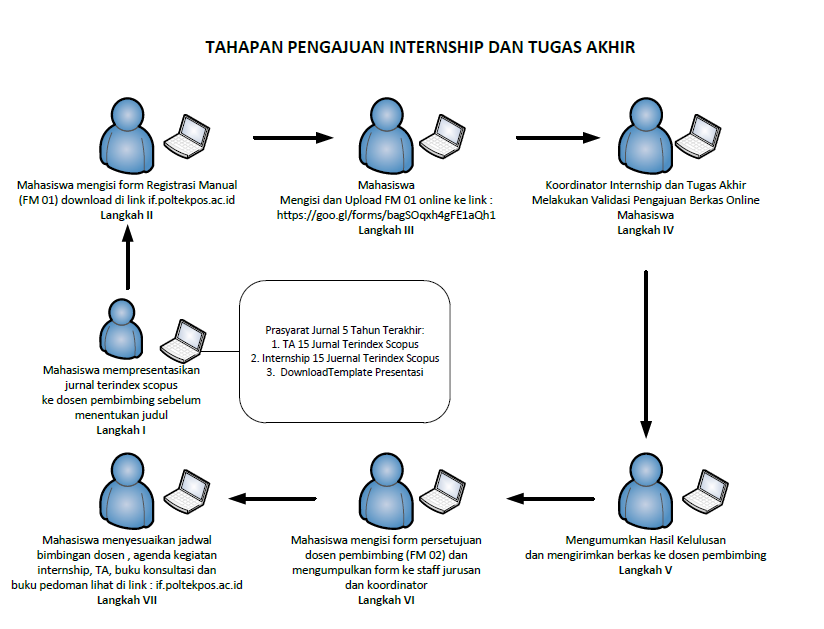
\includegraphics[width=1\textwidth]{figures/pengajuan.png}}
	\caption{Tahapan Pengajuan Judul Internship dan Tugas Akhir.}
	\label{figure:P1}
	\end{figure}


Penjelasan pada gambar  \ref{figure:P1} mahasiswa setelah bertemu dengan dosen pembimbing maka mengisi form 01 yang terdiri dari Judul dan Abstract.
\section{Judul}
Judul menggunakan bahasa Inggris. Judul diutamakan dapat menggambarkan riset dan metode yang akan dilakukan. Pemilihan judul juga harus dengan kesepakatan pembimbing. 

\section{Abstract}
Abstrak mengunakan bahasa inggris aktif dan positif. Tidak terdapat sitasi pada abstrak. Kalimat harus utuh terdiri dari Subjek Predikat Objek dan boleh ditambahkan Keterangan. Tidak boleh menggunakan kalimat pasif atau kalimat negatif. Abstrak harus terdiri dari 150-250 kata. Abstrak berisi latar belakang, tujuan, metode, dan target output dari penelitian.

\section{Ringkasan}
\subsection{Metode}
Metode yang digunakan adalah metode yang terdapat pada referensi dalam 5 tahun terakhir dari jurnal internasional terindex scopus. Penelitian harus menggunakan atau mengkombinasikan minimal 2 metode yang berbeda.

\subsection{Data Penelitian}
Sumber data penelitian harus ditargetkan dan jelas dari mana sumbernya. Sebutkan dari mana sumber datanya, berapa banyak datanya serta diskusikan bersama pembimbing mengenai jenis data apa saja yang harus didapatkan. 

\section{Referensi}
Semua referensi yang digunakan harus terindex pada google scholar. Minimal 15 referensi dari jurnal terindeks Scopus dan merupakan artikel dalam 5 tahun terakhir. Jurnal yang terindex scopus bisa dicek di situs scimagojr.com. Format referensi yang disikan pada formulir pengajuan penelitian tingkat akhir adalah BibTex. BibTex referensi bisa didapatkan pada laman Google Scholar.



